\subsection{Spielserver}
\label{sec:Spielserver}

Der Server bildet die Schnittstelle zwischen den beiden Kommunikationspartnern, indem er eingehende Nachrichten eines Clients an jeden anderen verbundenen Teilnehmer weiterleitet.
Des Weiteren limitiert er die maximale Spielerzahl und generiert das Startsignal, sobald sich zwei Teilnehmer mit ihm verbunden haben.
Außerdem legt das Programm fest, welcher der Spieler im Verteidigungs- bzw. Angriffsmodus startet.

Die Serverlogik wird maßgeblich durch die beiden Klassen \texttt{CCommunicationServer} und \texttt{CClientHandler} gesteuert (vgl. Abbildung \ref{fig:Serverklassendiagramm}).
Die Aufgabe der Klasse \texttt{CCommunicationServer} ist die Annahme eingehener Verbindungen.
Für jeden verbundenen Client wird ein separater Thread vom Typ \texttt{CClientHandler} erzeugt und gestartet.

Diese Threadobjekte führen die eigentliche Serverlogik aus.
Sie überwachen den eingehenden Datenstrom und sobald eine Nachricht eingegangen ist, wird diese kopiert und an jeden anderen Client weitergeleitet.
Für die Überwachung des Eingangsstromes ist die Methode \texttt{run()} verantwortlich und das Duplizieren der Nachricht wird in \texttt{notifyAllOtherClients(String line)} gehandhabt.
Der eigentliche Sendevorgang wird durch den Aufruf der Methode \texttt{send(String msg)} ausgeführt.

\begin{figure}[H]
  \centering
  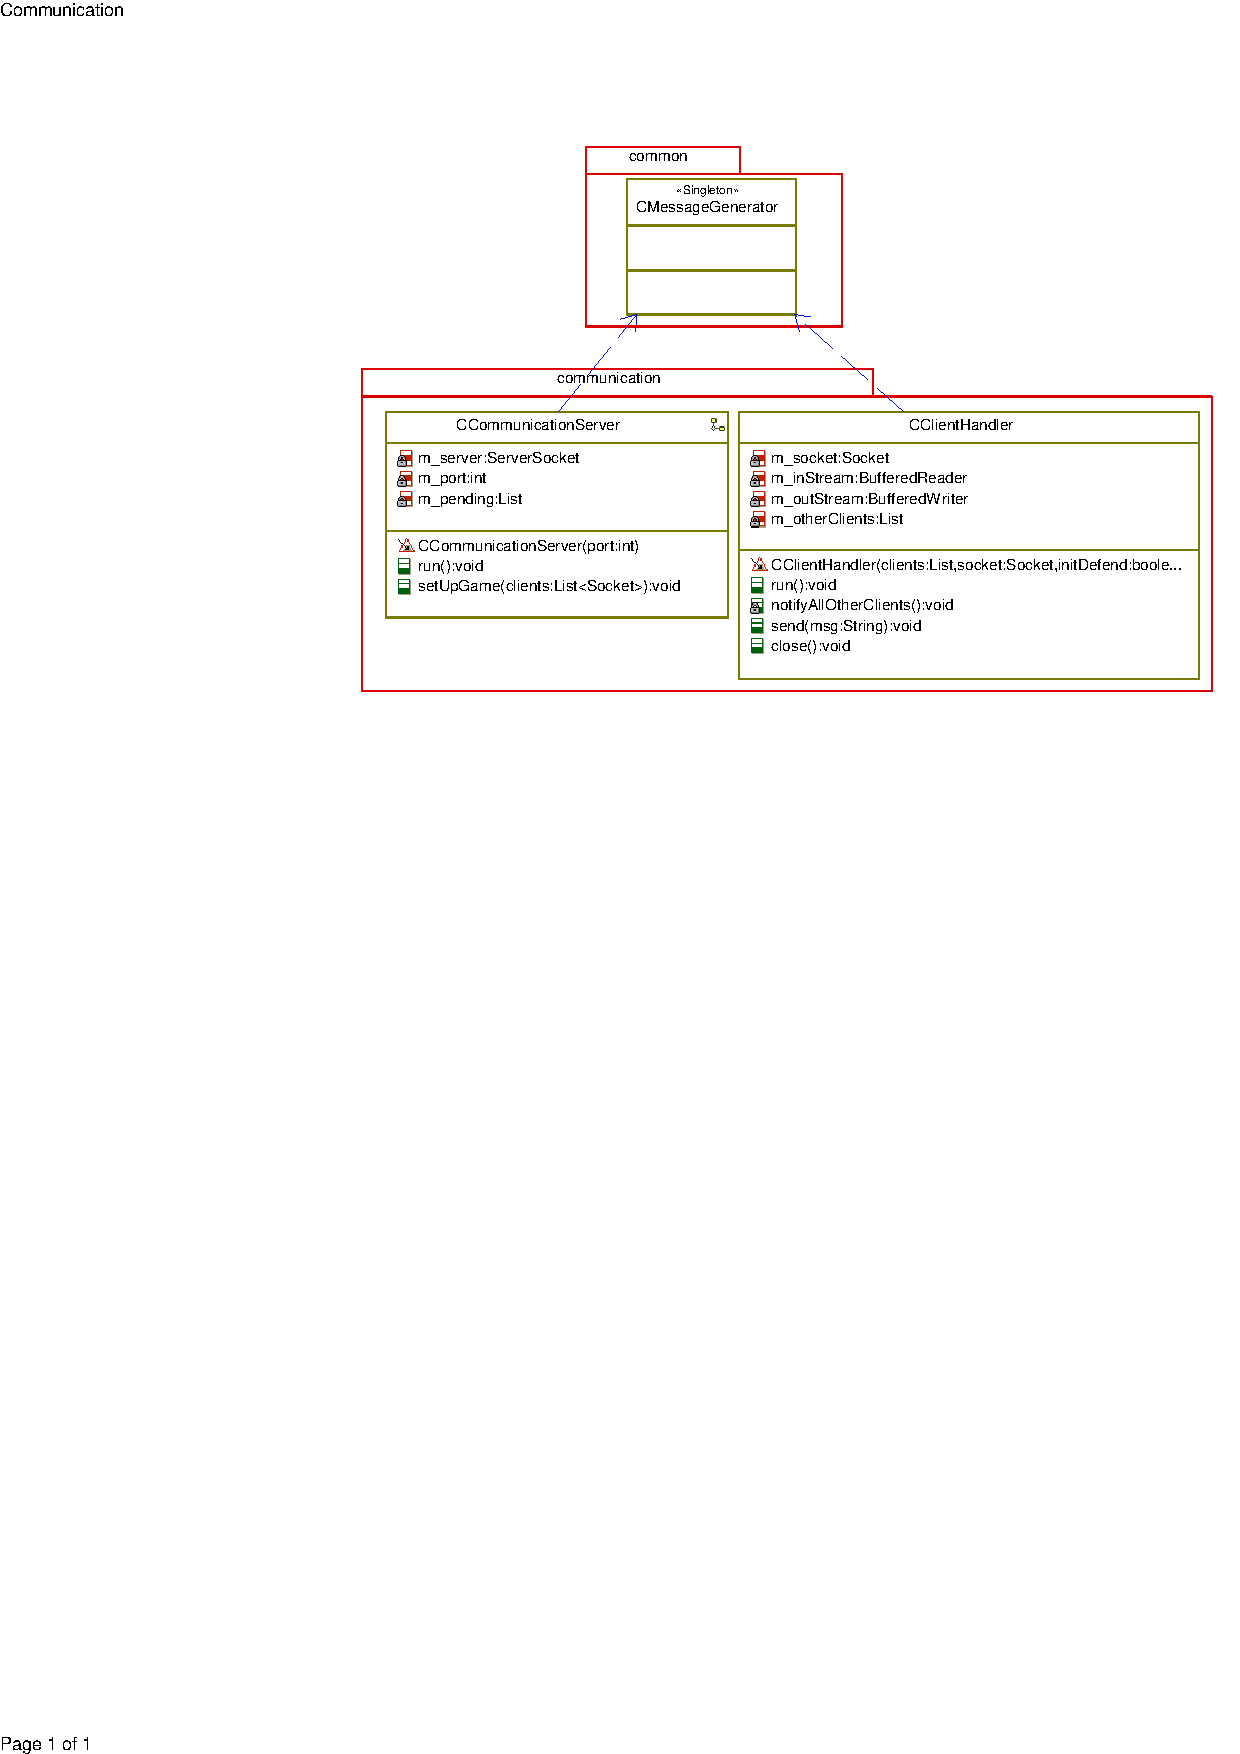
\includegraphics[trim=60mm 165mm 10mm 20mm,clip,width=0.8\textwidth]{images/Server.pdf}
  \caption{Klassendiagramm des Servers}
  \label{fig:Serverklassendiagramm}
\end{figure}
